% Options for packages loaded elsewhere
\PassOptionsToPackage{unicode}{hyperref}
\PassOptionsToPackage{hyphens}{url}
%
\documentclass[
  a4paper,
]{scrbook}

\usepackage{amsmath,amssymb}
\usepackage{iftex}
\ifPDFTeX
  \usepackage[T1]{fontenc}
  \usepackage[utf8]{inputenc}
  \usepackage{textcomp} % provide euro and other symbols
\else % if luatex or xetex
  \usepackage{unicode-math}
  \defaultfontfeatures{Scale=MatchLowercase}
  \defaultfontfeatures[\rmfamily]{Ligatures=TeX,Scale=1}
\fi
\usepackage{lmodern}
\ifPDFTeX\else  
    % xetex/luatex font selection
\fi
% Use upquote if available, for straight quotes in verbatim environments
\IfFileExists{upquote.sty}{\usepackage{upquote}}{}
\IfFileExists{microtype.sty}{% use microtype if available
  \usepackage[]{microtype}
  \UseMicrotypeSet[protrusion]{basicmath} % disable protrusion for tt fonts
}{}
\makeatletter
\@ifundefined{KOMAClassName}{% if non-KOMA class
  \IfFileExists{parskip.sty}{%
    \usepackage{parskip}
  }{% else
    \setlength{\parindent}{0pt}
    \setlength{\parskip}{6pt plus 2pt minus 1pt}}
}{% if KOMA class
  \KOMAoptions{parskip=half}}
\makeatother
\usepackage{xcolor}
\usepackage[right=2.54cm]{geometry}
\setlength{\emergencystretch}{3em} % prevent overfull lines
\setcounter{secnumdepth}{5}
% Make \paragraph and \subparagraph free-standing
\makeatletter
\ifx\paragraph\undefined\else
  \let\oldparagraph\paragraph
  \renewcommand{\paragraph}{
    \@ifstar
      \xxxParagraphStar
      \xxxParagraphNoStar
  }
  \newcommand{\xxxParagraphStar}[1]{\oldparagraph*{#1}\mbox{}}
  \newcommand{\xxxParagraphNoStar}[1]{\oldparagraph{#1}\mbox{}}
\fi
\ifx\subparagraph\undefined\else
  \let\oldsubparagraph\subparagraph
  \renewcommand{\subparagraph}{
    \@ifstar
      \xxxSubParagraphStar
      \xxxSubParagraphNoStar
  }
  \newcommand{\xxxSubParagraphStar}[1]{\oldsubparagraph*{#1}\mbox{}}
  \newcommand{\xxxSubParagraphNoStar}[1]{\oldsubparagraph{#1}\mbox{}}
\fi
\makeatother


\providecommand{\tightlist}{%
  \setlength{\itemsep}{0pt}\setlength{\parskip}{0pt}}\usepackage{longtable,booktabs,array}
\usepackage{calc} % for calculating minipage widths
% Correct order of tables after \paragraph or \subparagraph
\usepackage{etoolbox}
\makeatletter
\patchcmd\longtable{\par}{\if@noskipsec\mbox{}\fi\par}{}{}
\makeatother
% Allow footnotes in longtable head/foot
\IfFileExists{footnotehyper.sty}{\usepackage{footnotehyper}}{\usepackage{footnote}}
\makesavenoteenv{longtable}
\usepackage{graphicx}
\makeatletter
\def\maxwidth{\ifdim\Gin@nat@width>\linewidth\linewidth\else\Gin@nat@width\fi}
\def\maxheight{\ifdim\Gin@nat@height>\textheight\textheight\else\Gin@nat@height\fi}
\makeatother
% Scale images if necessary, so that they will not overflow the page
% margins by default, and it is still possible to overwrite the defaults
% using explicit options in \includegraphics[width, height, ...]{}
\setkeys{Gin}{width=\maxwidth,height=\maxheight,keepaspectratio}
% Set default figure placement to htbp
\makeatletter
\def\fps@figure{htbp}
\makeatother

%% Palatino font:
\usepackage[T1]{fontenc}
\usepackage[utf8]{inputenc}
\usepackage{palatino}

\usepackage{pifont}

\usepackage{upquote}

\usepackage{fontspec}
% % \usepackage[T1]{fontenc}
% \usepackage{tgbonum}

% % \newfontfamily\mytitlefont{\fontfamily{phv}\selectfont}
% \newcommand{\mytitlefont}{\fontfamily{phv}\selectfont}

% front page
\usepackage[colorlinks]{hyperref} % for text color on title
\usepackage{titling} % makes \thetitle etc available...
\usepackage{lipsum}
\usepackage{tikz}
\tikzstyle{bag} = [align=center] % allows new lines in text below
\AtBeginDocument{\thispagestyle{empty}
\definecolor{titlecolor}{HTML}{1C2404}
\begin{tikzpicture}[remember picture,overlay]
\draw (current page.center) node[inner sep=0] {\resizebox{!}{350mm}{\includegraphics{highres_banner.pdf}}};
\draw (current page.center) node[inner sep=0, opacity=0.5] {\resizebox{!}{100mm}{
\includegraphics{ausegl_sort.pdf}}};
% \draw (current page.center) node[bag] {  
        \draw (17, 1.7) node[bag, align=right, anchor=north east] {  
    % \mytitlefont 
    \color{titlecolor} \Large \textbf{Thesis} \\ 
    \\ 
    % \mytitlefont 
    \color{titlecolor} \Huge \textbf{\thetitle} \\ 
    \\ 
    % \mytitlefont
    \color{titlecolor} \huge \theauthor \\
    \\
    % \mytitlefont 
    \color{titlecolor} \Large \thedate 
    };
\end{tikzpicture}
\clearpage}

% back side
\AtEndDocument{\clearpage\thispagestyle{empty}
\begin{tikzpicture}[remember picture,overlay]
\draw (current page.center) node[inner sep=0] {\resizebox{!}{350mm}{\includegraphics{highres_banner.pdf}}};
% \draw (current page.center) node[bag] {  
    \draw (17, 1.7) node[bag, align=right, anchor=north east] {  
        % \mytitlefont 
        \color{titlecolor} \large Bioinformatics Research Centre \\ 
        % \mytitlefont 
        \color{titlecolor} \large Department of Molecular Biology and Genetics \\ 
        % \mytitlefont 
        \color{titlecolor} \large Aarhus University \\
        % \mytitlefont 
        \color{titlecolor} \large Universitetsbyen 81 \\
        % \mytitlefont 
        \color{titlecolor} \large 8000 Aarhus C \\
        % \mytitlefont 
        \color{titlecolor} \large Denmark
        };

\end{tikzpicture}}


% % picture (AU logo in title page)
% \usepackage{titlepic}
% % \usepackage{graphicx}
% \titlepic{\resizebox{!}{50mm}{
\includegraphics[width=\textwidth]{ausegl_sort.pdf}}}



% \pagestyle{plain} % no running header

\usepackage[many]{tcolorbox}
\definecolor{quotegray}{HTML}{505050}
\newtcolorbox{myquote}{%
    enhanced jigsaw, 
    breakable,      % allow page breaks
    frame hidden,   % hide the default frame
    left=1cm,       % left margin
    right=1cm,      % right margin
    colback=white,
    fontupper=\color{quotegray},
    overlay={%
        \node [scale=4,
            text=lightgray,
            inner sep=0pt,] at ([xshift=0.5cm,yshift=-0.7cm]frame.north west){``}; 
        \node [scale=4,
            text=lightgray,
            inner sep=0pt,] at ([xshift=-0.5cm]frame.south east){''};  
            },
        % paragraph skips obeyed within tcolorbox
                parbox=false,
}
% redefine the 'quote' environment to use this 'myquote' environment
\renewenvironment{quote}{\begin{myquote}}{\end{myquote}}

% add a dummy abstract environment that is defined in quarto manuscript 
% but not in the quarto book that we run first to give it a slot in the 
% side bar
\ifcsmacro{abstract}{}{
  \let\endmyenvironment\undefined%
  \newenvironment{abstract}{\chapter*{Abstract}}{}
}

% \usepackage{framed} % not sure i need this anymore

% \usepackage[T1]{fontenc}
% \usepackage{inconsolata}

% % I have to only define Shaded if it is already defined.
% % The reason is that pandoc does not define the macro if there are not code blocks in the a markdown file.
% \ifx \@Shaded \@empty

% \renewcommand{\KeywordTok}[1]{\textcolor[rgb]{0, 0, 0}{\textbf{{#1}}}} % def and or not reg
% \renewcommand{\BuiltInTok}[1]{\textcolor[rgb]{0.373, 0.298, 0.580}{\textbf{{#1}}}} % print open 
% \renewcommand{\VariableTok}[1]{\textcolor[rgb]{0.141, 0.392, 0.824}{\textbf{{#1}}}}
% \renewcommand{\OperatorTok}[1]{\textcolor[rgb]{0, 0, 0}{{#1}}} % def and or not reg
% \renewcommand{\DataTypeTok}[1]{\textcolor[rgb]{1.0,0.13,0.00}{{#1}}}
% \renewcommand{\DecValTok}[1]{\textcolor[rgb]{0.655, 0.498, 0.161}{{#1}}}
% \renewcommand{\BaseNTok}[1]{\textcolor[rgb]{0.259, 0.592, 0.596}{{#1}}}
% \renewcommand{\FloatTok}[1]{\textcolor[rgb]{0.655, 0.498, 0.161}{{#1}}}
% \renewcommand{\CharTok}[1]{\textcolor[rgb]{0.678,0.141,0.098}{{#1}}}
% \renewcommand{\StringTok}[1]{\textcolor[rgb]{0.678,0.141,0.098}{{#1}}}
% \renewcommand{\CommentTok}[1]{\textcolor[rgb]{0.135, 0.134, 0.133}{{#1}}}
% \renewcommand{\OtherTok}[1]{\textcolor[rgb]{0.00,0.44,0.13}{{#1}}}
% \renewcommand{\AlertTok}[1]{\textcolor[rgb]{1.00,0.00,0.00}{\textbf{{#1}}}}
% \renewcommand{\FunctionTok}[1]{\textcolor[rgb]{0.549, 0.102, 0.063}{\textbf{{#1}}}}  % function name
% \renewcommand{\RegionMarkerTok}[1]{{#1}}
% \renewcommand{\ErrorTok}[1]{\textcolor[rgb]{1.00,0.00,0.00}{\textbf{{#1}}}}
% \renewcommand{\NormalTok}[1]{\textcolor[rgb]{0, 0, 0}{{#1}}}


% \else
%   % no code blocks with markup...
% \fi



\usepackage{etoolbox}
\makeatletter
\g@addto@macro{\appendix}{%
  \patchcmd{\@@makechapterhead}% <cmd>
    {\endgraf\nobreak\vskip.5\baselineskip}% <search>
    {\hspace*{-.5em}:\space}% <replace>
    {}{}% <success><failure>
  \patchcmd{\@chapter}% <cmd>
    {\addchaptertocentry{\thechapter}}% <search>
    {\addchaptertocentry{Appendix~\thechapter:}}% <replace>
    {}{}% <success><failure>
  \addtocontents{toc}{%
    \protect\patchcmd{\protect\l@chapter}% <cmd>
      {1.5em}% <search>
      {6.5em}% <replace>
      {}{}}% <success><failure>
}
\renewcommand{\autodot}{}% Remove all end-of-counter dots
\makeatother


% restart chapter numbers in each part
\makeatletter
\@addtoreset{chapter}{part}
\makeatother


% \usepackage{chngcntr}
% \counterwithin*{subsubsection}{chapter}
% \counterwithout*{subsubsection}{section}
% \counterwithout*{subsubsection}{subsection}

% %  % KMT only use subsubsection number (this increments though the book 
% %  % when we supress numbering with  {.unnumbered} after each header except Exerisices
% \renewcommand\thesubsubsection{\arabic{section}}
% \renewcommand\thesubsubsection{\arabic{subsection}}
% \renewcommand\thesubsubsection{\arabic{chapter}-\arabic{subsubsection}}


\renewcommand*{\chapterformat}{%
  \textcolor[rgb]{0.7, 0.7, 0.7}{\thechapter}\autodot\enskip%
}
\renewcommand*{\sectionformat}{%
  \textcolor[rgb]{0.7, 0.7, 0.7}{\thesection}\autodot\enskip%
}
\renewcommand*{\subsectionformat}{%
  \textcolor[rgb]{0.7, 0.7, 0.7}{\thesubsection}\autodot\enskip%
}
\renewcommand*{\subsubsectionformat}{%
  \textcolor[rgb]{0.7, 0.7, 0.7}{\thesubsubsection}\autodot\enskip%
}



% % prevent latex from "floating" the figures
% \usepackage{float}
% \let\origfigure\figure
% \let\endorigfigure\endfigure
% \renewenvironment{figure}[1][2] {
%     \expandafter\origfigure\expandafter[H]
% } {
%     \endorigfigure
% }

\makeatletter
\@ifpackageloaded{caption}{}{\usepackage{caption}}
\AtBeginDocument{%
\ifdefined\contentsname
  \renewcommand*\contentsname{Table of contents}
\else
  \newcommand\contentsname{Table of contents}
\fi
\ifdefined\listfigurename
  \renewcommand*\listfigurename{List of Figures}
\else
  \newcommand\listfigurename{List of Figures}
\fi
\ifdefined\listtablename
  \renewcommand*\listtablename{List of Tables}
\else
  \newcommand\listtablename{List of Tables}
\fi
\ifdefined\figurename
  \renewcommand*\figurename{Figure}
\else
  \newcommand\figurename{Figure}
\fi
\ifdefined\tablename
  \renewcommand*\tablename{Table}
\else
  \newcommand\tablename{Table}
\fi
}
\@ifpackageloaded{float}{}{\usepackage{float}}
\floatstyle{ruled}
\@ifundefined{c@chapter}{\newfloat{codelisting}{h}{lop}}{\newfloat{codelisting}{h}{lop}[chapter]}
\floatname{codelisting}{Listing}
\newcommand*\listoflistings{\listof{codelisting}{List of Listings}}
\makeatother
\makeatletter
\makeatother
\makeatletter
\@ifpackageloaded{caption}{}{\usepackage{caption}}
\@ifpackageloaded{subcaption}{}{\usepackage{subcaption}}
\makeatother

\ifLuaTeX
  \usepackage{selnolig}  % disable illegal ligatures
\fi
\usepackage{bookmark}

\IfFileExists{xurl.sty}{\usepackage{xurl}}{} % add URL line breaks if available
\urlstyle{same} % disable monospaced font for URLs
\hypersetup{
  pdftitle={Title of my thesis},
  pdfkeywords={Blah blah, Blah blah, Blah blah},
  hidelinks,
  pdfcreator={LaTeX via pandoc}}


\title{Title of my thesis}
\usepackage{etoolbox}
\makeatletter
\providecommand{\subtitle}[1]{% add subtitle to \maketitle
  \apptocmd{\@title}{\par {\large #1 \par}}{}{}
}
\makeatother
\subtitle{Some subtitle for my thesis}
\author{Your Name}
\date{November 23, 2024}

\begin{document}
\frontmatter
\cleardoublepage
\thispagestyle{empty}
{\centering
\hbox{}\vskip 0cm plus 1fill
{%\mytitlefont 
\Huge\bfseries Title of my thesis \par}
\vspace{3ex}
{\Large\bfseries Some subtitle for my thesis \par}
\vspace{6ex}
{\Large\bfseries Your Name \par}
\vspace{3ex}
{\bfseries\large November 23, 2024 \par}
\vskip 0cm plus 2fill
{\resizebox{!}{50mm}{
\includegraphics[width=\textwidth]{ausegl_sort.pdf}} \par}
\vskip 0cm plus 2fill
{\bfseries\large Master of Science in Bioinformatics \par}
\vspace{3ex}
%
%
{\bfseries\large Aarhus University \par}
%
\vspace{12ex}
{\small Submitted in fulfillment of the requirements
of the degree of Master of Science in Bioinformatics \par}
\pagebreak
\begin{quote}
\raggedright    
Blah blah blah blah blah blah blah blah blah blah blah blah blah blah
blah blah blah blah blah blah blah blah blah blah blah blah blah blah
blah blah blah blah blah blah blah blah blah blah blah blah blah blah
blah blah blah blah blah blah blah blah blah blah blah blah blah blah
blah blah blah blah blah blah blah blah blah blah blah blah blah blah
blah blah blah blah blah blah blah blah blah blah blah blah blah.
\end{quote}
}

\renewcommand*\contentsname{Table of contents}
{
\setcounter{tocdepth}{1}
\tableofcontents
}

\mainmatter
\chapter{Introduction}\label{introduction}

Blah blah blah blah blah blah blah blah blah blah blah blah blah blah
blah blah blah blah blah blah blah blah blah blah blah blah blah blah
blah blah blah blah blah blah blah blah blah blah blah blah blah blah
blah blah blah blah blah blah blah blah blah blah blah blah blah blah
blah blah blah blah blah blah blah blah blah blah blah blah blah blah
blah blah blah blah blah blah blah blah blah blah blah blah blah.

\chapter{Methods}\label{methods}

Blah blah blah blah blah blah blah blah blah blah blah blah blah blah
blah blah blah blah blah blah blah blah blah blah blah blah blah blah
blah blah blah blah blah blah blah blah blah blah blah blah blah blah
blah blah blah blah blah blah blah blah blah blah blah blah blah blah
blah blah blah blah blah blah blah blah blah blah blah blah blah blah
blah blah blah blah blah blah blah.

\section{Sampling}\label{sampling}

Table~\ref{tbl-subjects} lists the samples included in the analysis.
Blah blah blah blah blah blah blah blah blah blah blah blah blah blah
blah blah blah blah blah blah blah blah blah blah blah blah blah blah
blah blah blah blah blah blah blah blah blah blah blah blah blah.

\begin{longtable}[]{@{}lllll@{}}

\caption{\label{tbl-subjects}People included in the analysis.}

\tabularnewline

\caption{}\label{T_41cb9}\tabularnewline
\toprule\noalign{}
name & age & sex & position & nationality \\
\midrule\noalign{}
\endfirsthead
\toprule\noalign{}
name & age & sex & position & nationality \\
\midrule\noalign{}
\endhead
\bottomrule\noalign{}
\endlastfoot
Julie & 27 & F & PhDstudent & DK \\
Thomas & 33 & M & Postdoc & GB \\
Emilie & 23 & F & PhDstudent & CH \\
Sofie & 31 & F & Postdoc & DK \\
Sara & 29 & F & Postdoc & US \\
Cecilie & 34 & F & Postdoc & DK \\
Anders & 32 & M & PhDstudent & UK \\
Emma & 42 & F & Professor & DK \\
Caroline & 31 & F & PhDstudent & DK \\
Laura & 30 & F & Postdoc & DK \\
Mikkel & 33 & M & Postdoc & NL \\
Jens & 27 & M & PhDstudent & DK \\
Andreas & 29 & M & PhDstudent & DK \\
Jakob & 28 & M & PhDstudent & DK \\
Mathilde & 61 & F & Professor & DK \\
Katrine & 35 & F & Postdoc & DK \\
Poul & 30 & M & Postdoc & DK \\
Anna & 26 & F & PhDstudent & DK \\
Peter & 42 & M & Professor & GB \\
Ida & 53 & F & Postdoc & DK \\
Freja & 30 & F & Postdoc & DK \\
Maria & 39 & F & Professor & UK \\
Amalie & 29 & F & PhDstudent & DK \\
Camilla & 35 & F & Postdoc & DK \\

\end{longtable}

\phantomsection\label{doc-sampling}
The 24 subjects from workplaces in Denmark were interviewed \ldots. blah
blah blah blah blah blah blah blah blah blah blah blah blah blah blah
blah blah blah blah blah blah blah blah blah blah blah blah blah blah
blah blah blah blah blah blah blah

Blah blah blah blah blah blah blah blah blah blah blah blah blah blah
blah blah blah blah blah blah blah blah blah blah blah blah blah blah
blah blah blah blah blah blah blah blah blah blah blah blah blah.

\section{Statistical analysis}\label{statistical-analysis}

Blah blah blah blah blah blah blah blah blah blah blah blah blah blah
blah blah blah blah blah blah blah blah blah blah blah blah blah blah
blah blah blah blah blah blah blah blah blah blah blah blah blah blah
blah blah blah blah blah blah blah blah blah blah blah blah blah blah
blah blah blah blah blah blah blah blah blah blah blah blah blah blah
blah blah blah blah blah blah blah.

\subsection{Clustering}\label{clustering}

Blah blah blah blah blah blah blah blah blah blah blah blah blah blah
blah blah blah blah blah blah blah blah blah blah blah blah blah blah
blah blah blah blah blah blah blah blah blah blah blah blah blah blah
blah blah blah blah blah blah blah blah blah blah blah blah blah blah
blah blah blah blah blah blah blah blah blah blah blah blah blah blah
blah blah blah blah blah blah blah.

\subsection{Linear models}\label{linear-models}

Blah blah blah blah blah blah blah blah blah blah blah blah blah blah
blah blah blah blah blah blah blah blah blah blah blah blah blah blah
blah blah blah blah blah blah blah blah blah blah blah blah blah blah
blah blah blah blah blah blah blah blah blah blah blah blah blah blah
blah blah blah blah blah blah blah blah blah blah blah blah blah blah
blah blah blah blah blah blah blah.

\chapter{Results}\label{results}

As shown in Figure~\ref{fig-danish-interaction}, blah blah blah blah
blah blah blah blah blah blah blah blah blah blah blah blah blah blah
blah blah blah blah blah blah blah blah blah blah blah blah blah blah
blah blah blah blah blah blah blah blah blah blah blah blah blah.

\begin{figure}[H]

\centering{

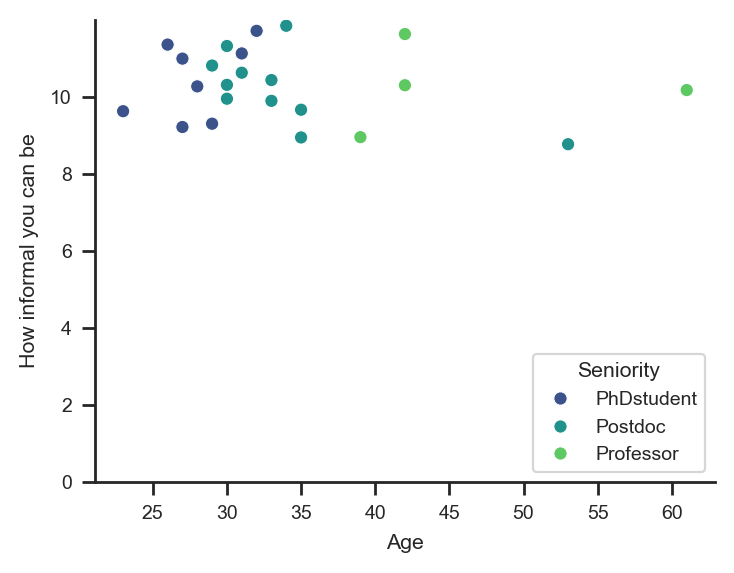
\includegraphics[width=3.82292in,height=2.97917in]{index_files/figure-latex/..-notebooks-example-fig-danish-interaction-output-1.png}

}

\caption{\label{fig-danish-interaction}Interaction among Danes: How
Danes interact is has very little to do with age and seniority, compared
to most other contries.}

\end{figure}%

As shown in Figure~\ref{fig-meaninformality}, \ldots{} blah blah blah
blah blah blah blah blah blah blah blah blah blah blah blah blah blah
blah blah blah blah blah blah blah blah blah blah blah blah blah blah
blah blah blah blah blah blah blah blah blah blah blah blah blah blah.

\begin{figure}[H]

\centering{

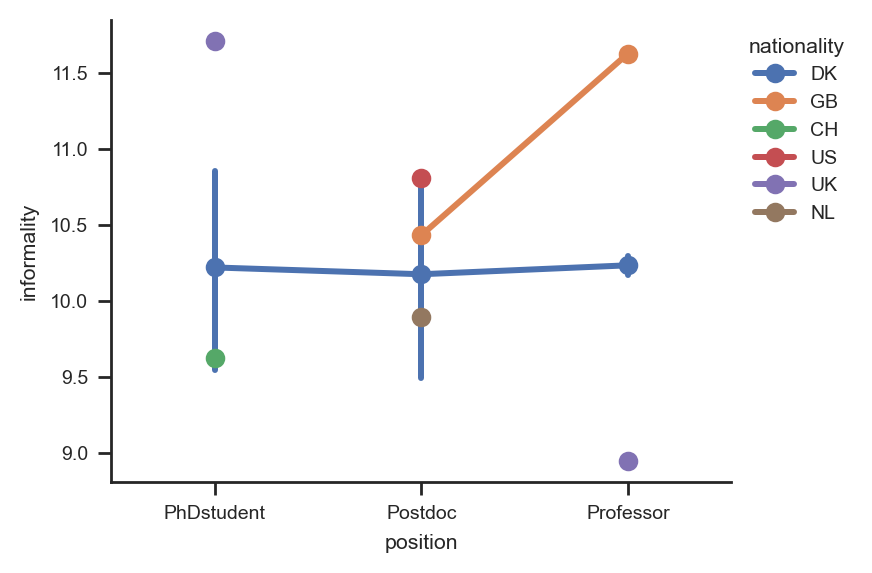
\includegraphics[width=4.45833in,height=2.97917in]{index_files/figure-latex/..-notebooks-example-fig-meaninformality-output-1.png}

}

\caption{\label{fig-meaninformality}Mean interaction scores by position
and nationality.}

\end{figure}%

Blah blah blah blah blah blah blah blah blah blah blah blah blah blah
blah blah blah blah blah blah blah blah blah blah blah blah blah blah
blah blah blah blah blah blah blah blah blah blah blah \ldots{}
Table~\ref{tbl-meaninformality} lists the mean interaction scores by
position and nationality.

\begin{longtable}[]{@{}lll@{}}

\caption{\label{tbl-meaninformality}Mean interaction scores by position
and nationality.}

\tabularnewline

\caption{}\label{T_42276}\tabularnewline
\toprule\noalign{}
position & nationality & informality \\
\midrule\noalign{}
\endfirsthead
\toprule\noalign{}
position & nationality & informality \\
\midrule\noalign{}
\endhead
\bottomrule\noalign{}
\endlastfoot
Professor & GB & 8.086033 \\
Professor & UK & 9.590511 \\
Postdoc & DK & 9.880289 \\
Postdoc & GB & 9.949350 \\
Postdoc & US & 10.366486 \\
PhDstudent & DK & 10.608510 \\
PhDstudent & CH & 10.751572 \\
Postdoc & NL & 11.244057 \\
PhDstudent & UK & 11.322927 \\
Professor & DK & 12.400968 \\

\end{longtable}

\subsection{Subsubsection}\label{subsubsection}

Blah blah blah blah blah blah blah blah blah blah blah blah blah blah
blah blah blah blah blah blah blah blah blah blah blah blah blah blah
blah blah blah blah blah blah blah blah blah blah blah blah blah blah
blah blah blah blah blah blah blah blah blah blah blah blah blah blah
blah blah blah blah blah blah blah blah blah blah blah blah blah blah
blah blah blah blah blah blah blah.

\chapter{Bon mot}\label{bon-mot}

\begin{quote}
Nothing in Biology Makes Sense except in the Light of Evolution

- Theodosius Dobzhansky
\end{quote}

\chapter{References}\label{references}


\backmatter


\end{document}
